\documentclass[10pt,a4paper]{article}
\usepackage[utf8]{inputenc}
\usepackage{amsmath}
\usepackage{amsfonts}
\usepackage{amssymb}
\usepackage{fullpage}
\usepackage{verbatim}
\usepackage{graphicx}
\begin{document}

\title{Crowd density estimation from Wi-Fi positioning data in the Amsterdam Arena}
\maketitle

\begin{abstract}
\begin{comment}
We present the Amsterdam Arena project, which involves observing and managing crowd behaviour, using the Amsterdam Arena stadium as a living laboratory. The main scientific question we explore is how to detect anomalous behaviour in large crowds in real time. The main purpose is to be able to predict a possible crowd disaster and identify means to prevent it from happening. 
Human crowds are complex systems, and predicting or controlling their behaviour is challenging. Our approach involves three phases, firstly data collection from Wi-Fi and Bluetooth sensors in the stadium, secondly data analytics, and finally we aim to use simulation to make forecasts about the crowd dynamics. 
Here we present initial results on the data analytics and show how we can extract density maps from Wi-Fi positioning data. The technology we deploy is based on the Wi-Fi signals from smart phones. We use the existing network of Wi-Fi access points in the stadium, and capture probe signals from smart phones, which are processed and anonymised in alignment with privacy concerns. The positions of smart phones are reconstructed using received signal strengths and methods similar to trilateration. The data provides us with real-time information on spatial distributions of crowd density, which is an essential indicator of the criticality of crowd conditions. To visualise the spatiotemporal behaviour of crowd density in real-time we dynamically generate heat maps along a moving time interval. The heat maps are generated through the statistical modelling of the positioning data. The generation of dynamic heat maps allows us to detect and locate hot-spots of density where crowd conditions reach critical values that could possibly lead to a disaster.
\end{comment}
\end{abstract}

\section{Introduction}


***********************************From Sonja. nb: the text will be polished in the final phases, first I care only about putting all ideas on paper***************

Crowd disasters have taken many human lives. The Love Parade disaster (Duisburg, 2010), the Ellis Park Stadium disaster (Johannesburg, 2001), the PhilSports Stadium stampede (Manila, 2006) are just a few recent examples. One of the reasons that disasters happen is a "lack of overview of everybody" [cite paper on love parade EPJ DS], that is, a lack of macroscopic overview of the crowd. Critical crowd density (cite paper 8/m2, find it in e-mails)) is a contributing factor to crowd disasters; yet, it is still challenging to determine timely when it occurs, so that a disaster can be prevented before it happens, by e.g. navigating the rest of the crowd away from the congestion. 

In our work we are interested in estimating crowd density during concerts in indoor spaces. A lot of research on estimating crowd density has been done using video processing from security cameras (cite papers (1), (2), (3) from proposal?). However, this approach does not apply in our case, because 1)  it is difficult to obtain macroscopic overview ; 2) the lighting conditions during concert hours are not sufficient for video-based crowd analysis; and 3) the error of video-based density estimation increases with the increase of the actual crowd density.  

In our approach, we combat the three above mentioned issues by exploiting the ubiquity of smart phones, as in ((4) (5), (6) from proposal?). Our living laboratory is the Amsterdam Arena(citation). Or methodology consists of three steps.  First, we are using the Wi-Fi routers in the stadium to gather the strengths of the wireless antena signals from individuals smart phones.  Second, we are estimating anonymously the positions of the visitors from the signal strengths in real time. This technique has been presented in (cite Jan's slides), and is similar to trilateration, that is, the way the Global Positioning System (GPS) is implemented. However, due to signal interference and blockage in dense crowds, irregular internet packet rates and systematic errors leading to multiple local optima, the positioning itself does not suffice to estimate the crowd density. Thus, in our third step, we aggregate the results from the positioning and apply the law of the large numbers to obtain an estimation of the crowd density, also in real-time. With the first two steps, we are dealing with issues 1) and 2) mentioned above. With the third step, which is the main contribution of this paper, we are handling issue 3) -  that is, with our method the precision of estimation actually increases as the crowd density increases. 

The rest of the paper is organized as follows.....******* 

*************n.b. in related work section put all that use wi-fi tracking, for those that use GPS tracking only mention that this does not work in indoor spaces and that it requires participation. Not necessary to put work on video tracking in related work - it is already mentioned in intro. Mention also bluetooth tracking, but bluetooth is not so ubiquitous and our principles apply also if bluetooth was used (right?) 
Finally, none of the mentioned work uses our approach of modeling the position of an individual as a probability distribution; our method is designed to attack the problem of having a dense crowd; we are not interested in precise estimations for freely moving crowds; rather, we are interested in obtaining precise estimation when the  concert crowds is dense and static due to this. blah blah (sonja: explain better)********

************************************end from Sonja
\begin{comment}
\begin{itemize}

\item Background\\

Human crowds are complex systems, and predicting or controlling their behavior is challenging. Our approach involves three phases, firstly data collection from Wi-Fi and Bluetooth sensors in the stadium, secondly data analytics, and finally we aim to use simulation to make forecasts about the crowd dynamics. 

In this paper we present initial results on the data analytics and show how we can extract density maps from Wi-Fi positioning data. 

\item Aims\\

The main purpose is to be able to predict a possible crowd disaster and identify means to prevent it from happening. 

\end{itemize}
\end{comment}

\section{Positioning of visitors using Wi-Fi sensors and smart phones}


This section will be written later, maybe with input from Jan.

\begin{comment}
The technology we deploy is based on the Wi-Fi signals from smart phones. We use the existing network of Wi-Fi access points in the stadium, and capture probe signals from smart phones, which are processed and anonymised in alignment with privacy concerns. The positions of smart phones are reconstructed using received signal strengths and methods similar to trilateration. 


\begin{itemize}
\item How are the uncertainties (errors) generated and what do they mean?
\end{itemize}
\end{comment}
\section{From positioning to estimation of density}



Sonja:Mention somewhere that in the documentary of the LP disaster people were raising their phones up to look for a way out. (which is good , less blockage of signals)
\subsection{Issues with positioning (title to reconsider)}

Under ideal circumstances, the positioning itself would suffice to estimate the crowd density per region of interest:  every few seconds we would only need to count the number of estimates that fall in the region of interest. However, we have observed several issues, which are not related to the mathematical methodology behind the positioning step, that prevent us to apply direct counting. 
\begin{enumerate}
	\item
	{\it Multiple local optima}. Due to signal interference, when the optimization of the estimation of location of a certain MAC address is performed, there can be multiple local optima that are equally good candidates. For example, consider Fig. \ref{fig:trilateration_problem} \footnote{Picture courtesy of http://math.stackexchange.com/questions/42537/trilateration-with-bounds}. In the center of every ring there is a Wi-Fi router, that has estimated signal strength to a certain MAC device with a certain error range. The error range is represented by the thickness of the ring. Then, there are two possible regions which are equally good candidates for the positioning of the MAC device, and those regions are the two darkest regions where all three rings overlap. Note that the problem can arise regardless of the thickness of the rings or the number of Wi-Fi routers. 	
	\begin{figure}[h!]
		\centering
		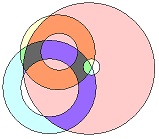
\includegraphics[width=40mm]{trilateration_problem.jpg}
		\caption{Trilateration can lead to multiple local optima}
		\label{fig:trilateration_problem}
	\end{figure}
	In fact, let us consider a static (24 hours persistent) MAC device.  We have  plotted the estimations of its coordinates through time, where we have plotted only the estimations with a relatively small error  (Fig. \ref{fig:bimodal})
	\begin{figure}[h!]
		\centering
		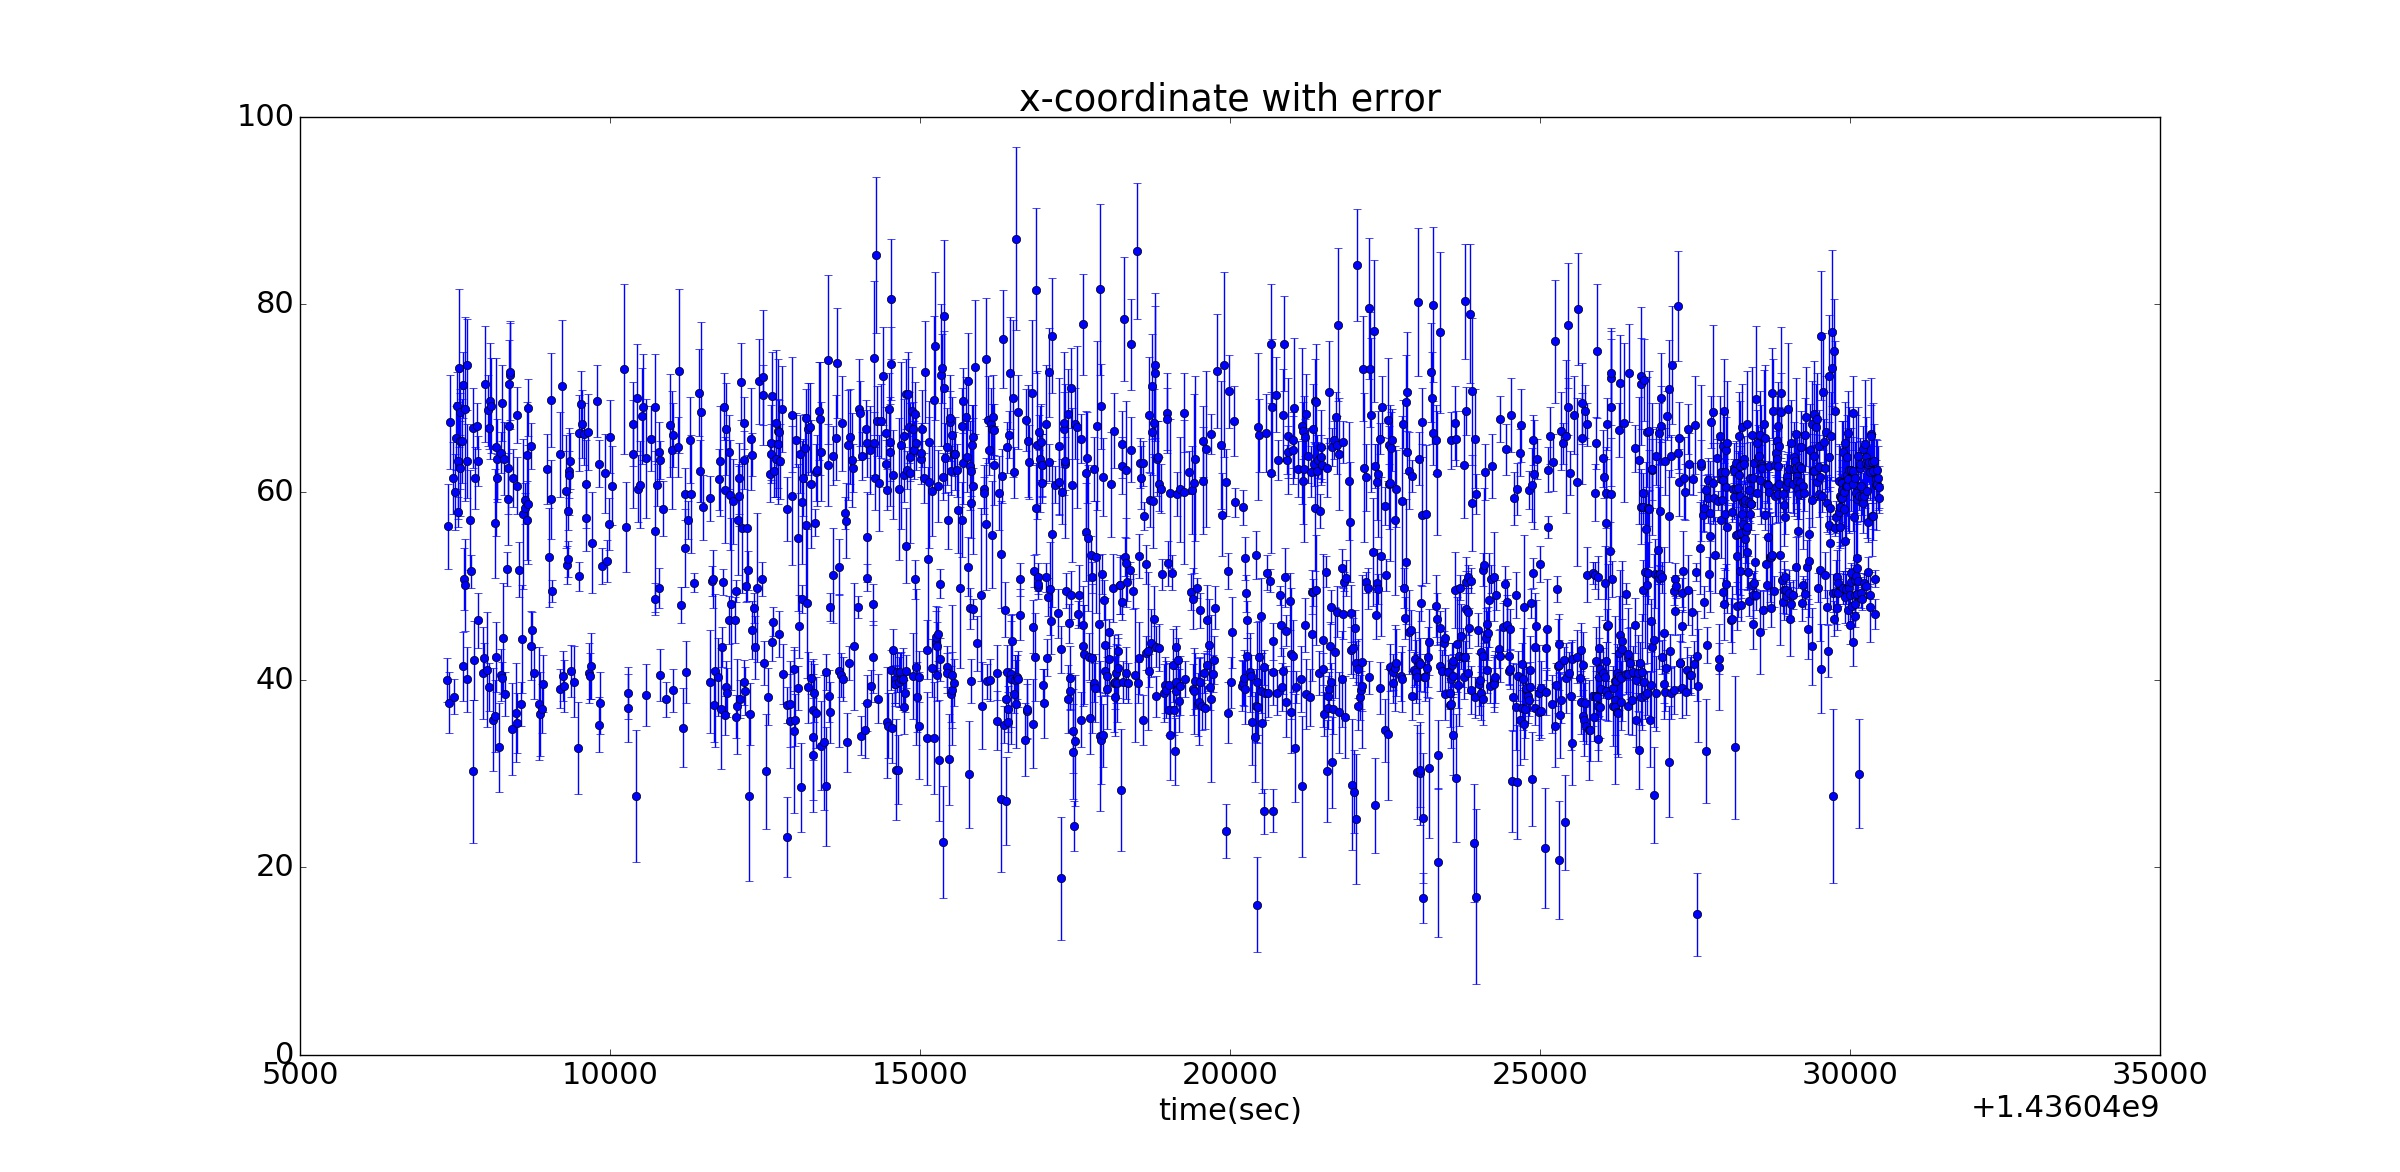
\includegraphics[width=100mm]{bimodal.jpg}
		\caption{Trilateration can lead to multiple local optima (cut the lower part from the picture)}
		\label{fig:bimodal}
	\end{figure} 
	The resulting plot (for the x-coordinate) reveals a bimodal distribution of the estimation. We have observed such a distribution in a majority of the 20 randomly sampled MAC addresses. This phenomenon can be explained by the multiple local optima situation, because we did not observe bi-modal distributions in the signal strengths. 
	
\item {\it Volatility of packet rates}. When a MAC device is connected to the WI-Fi internet, it sends packets with a relatively stable rate. However, during concert hours, very few devices are actually connected to the internet, and most of our estimations of positions come from signals that the device sends in a "probing" mode. In this case the packet rate is quite volatile, ranging from a few seconds to a few minutes (some citation?). This means that when we make a snapshot of the MAC addresses visible in a certain moment, we are only detecting a small fraction of the MAC devices.   

\item {\it MAC randomization}. Due to ever increasing privacy concerns and possibly other business reasons, starting from 2014, the Apple I-phones have introduced randomization of the MAC address when the device is in a probing mode (not connected to internet) (citation?). This means that when the device switches from a probing to an online mode or vice versa, the MAC address suddenly changes and thus the device cannot be followed anymore. (n.b. here or later: there is a tag that reveals whether the address is randomized or not)    
\end{enumerate}


\subsection{Addressing the issues: real-time crowd density estimation}

\begin{comment}
To visualise the spatiotemporal behaviour of crowd density in real-time we dynamically generate heat maps along a moving time interval. The heat maps are generated through the statistical modeling of the positioning data. The generation of dynamic heat maps allows us to detect and locate hot-spots of density where crowd conditions reach critical values that could possibly lead to a disaster.
\end{comment}

\begin{itemize}
\item The method we use is similar to Kernel Density Estimation, but what we are doing is not actual smoothing (?).
\end{itemize}

To construct two-dimensional probability density functions we apply non-parametric density estimation.
To make density histograms we consider a two-dimensional binned region of space, and count the number of positions that fall into each bin. For each bin location $X$, in the time interval $t$, we apply the kernel density estimation (KDE) method \cite{scott}\cite{silverman} given by

\begin{equation}
\hat{d}(X,t)=\frac{1}{N }\sum_{i=1}^{N} K_{h_{x}} (x-x_{i}) K_{h_{y}} (y-y_{i})
\label{kde}
\end{equation}

where $K_{h_{u}}$ is the kernel function $K_{h}(u)=K(u/h)/h$, $h$ is the smoothing parameter, or bandwidth, and $N$ is the number of data points (positions) in the time interval $t$.

The bandwith parameter $h$ is crucial for the accuracy of the density estimate. 
Several theoretical approaches are possible.
Here we base our choice of kernel bandwidth values $h$ on the error values $(\sigma_{x},\sigma_{y})$ provided by the positioning methods (see Section ).

\subsection{Real-time data analysis}

To process positioning data in real-time during events, we consider data within a specific moving time window.
To take in account that visitors are moving, we subdivide the time window in multiple sub-windows and attach more weight to measurements in later sub-windows. The weighting scheme is given by

\begin{equation}
\hat{d}(X,t)=\frac{w_{1}\hat{f}(X,t_{1})+w_{2}\hat{f}(X,t_{2})+...+w_{m}\hat{f}(X,t_{m})}{w_{1}N_{1}+w_{2}N_{2}+...+w_{m}N_{m}}
\end{equation}

\noindent where $\hat{f}(X,t)$ is the non-normalized sum of smoothed counts ($N\times\hat{d}(X,t)$) in Equation \ref{kde}, $w_{k}$ is the weight value given to sub-window $k$, and $m$ is the number of sub-windows.

\subsection{Validation}

\begin{itemize}
\item Simulation?\\
Do we include simulation of the positioning process, i.e. the toy Monte Carlo simulation, or do we generate fitted positions with error values, and only test the density estimation methods?
\end{itemize}

\section{Related work}

Wirz \textit{et al.} (2012) \cite{wirz:1} infer crowd density from GPS location traces of people who use an App during the 2011 Lord Mayor Show in London. They visualize the data in real-time, and generate heat maps (dynamically) using the kernel density estimation (KDE) method. In (Wirz \textit{et al.} 2013) \cite{wirz:2} the methodology is presented more elaborately, using a real-world data set collected during the same festival. The relation between the number of App users and the crowd density is calibrated (using linear regression), which forms the basis of their participatory sensing method. 
The accuracy of the smoothing method is assessed using ground truth crowd density information obtained from video footage recorded by CCTV cameras. 
The influence of the kernel radius on the correlation between the actual density and the density of App is analysed.

The Gaussian weight function used in (Wirz \textit{et al.} 2012; 2013) \cite{wirz:1}\cite{wirz:2} is introduced in Helbing \textit{et al.} (2007) \cite{helbing:1} to estimate local densities in an area captured by video cameras during the Hajj in Mina/Makkah in 1426H on January 12, 2006.\\

A number of studies use Bluetooth to estimate crowd densities at a wide range of places and events.
In these studies the position of a mobile phone is approximated to the location of the sensor by which it is detected.

Schauer \textit{et al.} (2014) \cite{schauer:1} count unique MAC addresses detected by two sensors (nodes) at both sides (public and security) of a security check inside a major German airport, to estimate pedestrian densities and pedestrian flow. They consider time information, to determine the direction of a person's movement, and at least one RSSI value, to reduce the number of false positives in case devices are captured by both sensors. They compare Bluetooth and Wi-Fi based methods, and compare their methods to a known ground truth provided by the number of security checks.

Versichele \textit{et al.} (2012) \cite{versichele:1} use Bluetooth scanners at strategic locations during the 10-day Ghent Festivities, to analyze spatio-temporal dynamics of pedestrians. 

Yoshimura \textit{et al.} (2016) \cite{yoshimura:1} use Bluetooth detection to analyze visitors' behavior at the Louvre museum in Paris.

Delafontaine \textit{et al.} (2012) \cite{delafontaine:1} use a similar approach (of Bluetooth tracking) and apply (genetic) sequence alignment methods to analyze the resulting data which consists of different sequences of sensors (nodes) for detected mobile devices.

Weppner and Lukowicz (2013) \cite{weppner:1} estimate crowd densities during a soccer European championship public viewing event and during the Oktoberfest, by distributing volunteers in the crowd, who are carrying smart phones scanning for Bluetooth devices. They then use statistics to combine the different measurements in space and time.

In Weppner \textit{et al.} (2014) \cite{weppner:2} similar methods are applied to a city-wide festival in Zurich 2013, now supported by GPS data.



\section{Conclusion}



\bibliography{references}
\bibliographystyle{plain}

\end{document}